\section{Analyse approfondie du cas}

\subsection{Use-case}
Dans le cadre de la gestion de l'agence immobilière, nous avons pointé les grandes fonctionnalités du système. Ces grandes fonctionnalités représentent les interactions des acteurs avec le système.
Elles sont les suivantes :
\begin{itemize}
	\item l'ajout d'une personne,
	\item l'ajout d'un bien,
	\item la gestion d'une demande d'un client,
	\item la planification des visites,
	\item l'établissement d'un contrat
	\item la création de statistiques.
\end{itemize}
Pour chacune de ces grandes fonctionnalités, nous avons réalisé un scénario précisant le fonctionnement du point de vue de l'agence. En effet, les acteurs du système sont exclusivement représentés par le personnel de l'agence.
Toutefois, ces scénarios sont basés sur la perception du client.\\

\begin{figure}[H]
\centering
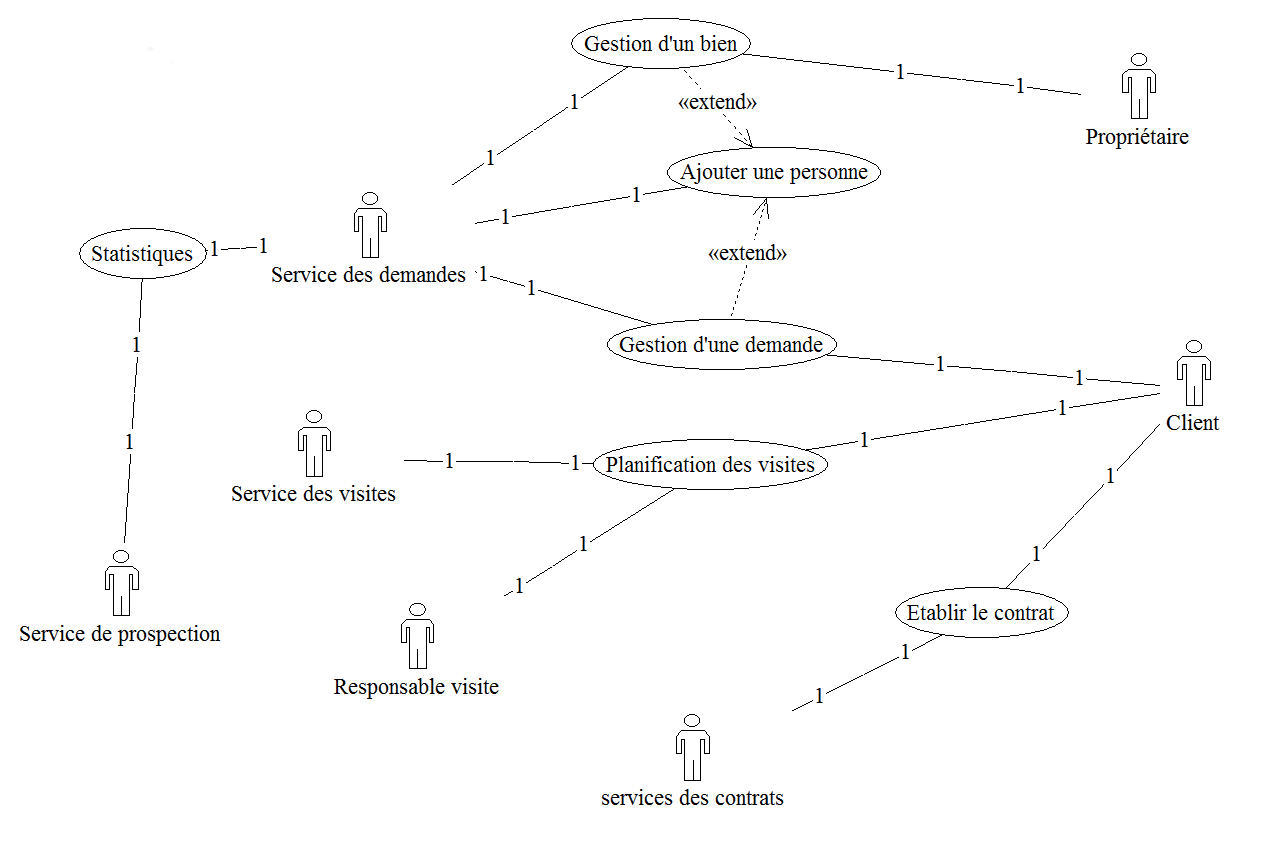
\includegraphics[width=16cm]{use-case.png}
\caption{Use-case diagram, réalisé à l'aide de DB-Main}
\label{fig:diagUC}
\end{figure}

Les scénarios que nous avons découvert sont repris ci-dessous. Ceux-ci nous ont permis de mieux concevoir la manière dont fonctionne une agence immobilière, et nous ont donc aidé dans la complétion et a vérification de notre schéma entité-association. En plus des scénarios par après, vous trouverez dans la figure \ref{fig:diagUC} un schéma représentant les scénarios et les acteurs de ceux-ci.

\subsubsection{L'ajout d'une personne}
Par personne, nous entendons aussi bien le client désireux d'acheter ou louer un bien que le propriétaire souhaitant vendre ou louer son bien.
La procédure d'ajout est directement liée à la demande de recherche d'un bien et à l'enregistrement d'un bien.

Tout d'abord, l'employé saisit le nom, le prénom, l'adresse de la personne.
Le système vérifie que l'adresse n'existe pas déjà à l'intérieur de celui-ci et assure l'unicité de cette personne. L'unicité se fait sur le nom, le prénom et l'adresse.
Le système enregistre ces informations et assigne un identifiant par compostage. Notons que les identifiants des propriétaires commencent tous par P, ceux des clients par C, et ceux des agents (non concernés ici), par A.
Enfin, l'employé demande les numéros de téléphone de la personne, ainsi que ses heures de disponibilité afin que le système les enregistre.

\subsubsection*{Tableau récapitulatif}
\begin{longtable}{|p{7.5cm}|p{7.5cm}|}
\hline
Acteur (service des demandes) & System\\
\hline
1. Encode le nom, le prénom, l'adresse & 2. Enregistre le nom et le prénom\\
& 3. vérifie l'existence de l'adresse dans le système d'information\\
& 4. Vérifie l'unicité de la nouvelle personne\\
& 5. Enregistre le propriétaire\\
6. Encode les numéros de téléphone  & 7. Enregistre les numéros de téléphone\\
\hline
\end{longtable}
\subsubsection{L'ajout d'un bien}
Lorsqu'un propriétaire se présente à l'agence, il se rend auprès du service des demandes.
Ce service commence par saisir les informations relatives à ce propriétaire.
Ensuite, le système vérifie l'existence de ce propriétaire. S'il existe l'employé continue son travail en saisissant les informations relatives au bien. Dans le cas contraire, il commence tout d'abord par ajouter le propriétaire dans le système, pour ensuite saisir les informations relatives au bien.

Pour le bien, l'employé commence par saisir les informations sur le type de bien (maison, appartement, etc.), le mode d'offre (vente/location), le montant/loyer demandé et la superficie.
À la suite de cela, le système détermine la classe standard à laquelle appartient le bien.
Si aucune classe standard ne peut être associée, le système accepte tout de même le bien et le range dans une classe "en attente".
Maintenant que le bien possède sa classe standard, l'employé peut saisir les informations relatives au bien à l'aide des champs optionnels disponibles pour celle-ci.
Ces champs sont dépendants de la classe standard, car les informations nécessaires ne sont pas les mêmes selon le type du bien et le mode d'offre.

\subsubsection*{Tableau récapitulatif}
\begin{longtable}{|p{7.5cm}|p{7.5cm}|}
\hline
Acteur (service des demandes)& System\\
\hline
1. Saisit les identifiants du propriétaire & 2. Vérifie l'existence de ce propriétaire\\
3. S'il n'existe pas, encode le nouveau propriétaire & 4. Enregistre le propriétaire\\
5. Encode le type de bien, le mode d'offre, le prix demandé et la superficie & 6. Attribue la classe standard correspondant au bien\\
7. Encode les informations complémentaires correspondant à la classe standard & 8. Enregistre ces informations\\	
\hline
\end{longtable}
\subsubsection{La gestion de la demande d'un client}
Le client acheteur/locataire s'adresse au service des demandes.
Ce service va assister le client dans sa recherche de bien en lui présentant les biens correspondants à ses critères.
Pour ce faire, l'employé regarde si le client est déjà inscrit auprès de l'agence. Dans le cas où il ne serait pas inscrit, l'employé ajoute ce dernier dans le système.

Ensuite, il demande le type de bien, ainsi que le mode d'offre qui intéressent le client, et enfin son budget et la superficie minimum souhaitée pour le bien. Le système détermine alors les classes standards qui pourraient convenir aux souhaits du client.
Pour sélectionner uniquement les biens, l'employé encode les choix du client pour les éléments optionnels, par exemple le nombre de chambres, la présence d'un jardin, etc.

Suite à cela, le système imprime la liste des biens disponibles correspondants aux différents critères du client.
Sur cette liste, le système imprime  la localisation du bien, le prix demandé et la superficie.
A partir de cette liste, le client va opérer un premier tri avec l'employé, qui éliminera de la liste les biens non-désirés.

Finalement, le client reçoit la liste des biens qu'il a sélectionnés.

\subsubsection*{Tableau récapitulatif}
\begin{longtable}{|p{7.5cm}|p{7.5cm}|}
\hline
Acteur (service des demandes)& System\\
\hline
1. Encode le type de bien, le mode d'offre, le budget (la superficie minimale souhaitée, éventuellement) du client & 2. Cherche les classes standard correspond aux critères\\
3. Encode les caractéristiques supplémentaires recherchées par le client & 4. Cherche la liste des biens disponibles correspondants aux critères du client\\
& 5. Imprime la liste (localisation, prix demandé, info superficie)\\
6. Encode les choix du client & 7. Enlève de la liste les biens non souhaités\\
\hline
\end{longtable}

\subsubsection{La planification des visites}
Pour la gestion des plannings des visites, le service des visites reçoit les demandes de la part des clients.
Les clients se présentent avec la liste des biens qu'ils ont sélectionnés au préalable avec le service des demandes.
Cette liste est analysée par les employés du service des visites. L'un des employés interroge le système d'information pour obtenir des informations plus détaillées sur les biens. Un autre employé interroge le système afin d'obtenir les photos des différents biens.
À l'aide les photos et les informations détaillées, le client opère un deuxième tri avec le service des visites. À le fin de ce tri, l'employé supprime de la liste du client les biens non-désirés.

Le service des visites affiche le planning des visites pour les biens restants.
En fonction de ses disponibilités et des plages horaires restantes, le client transmet à l'employé les plages horaires qui l'intéressent. L'employé enregistre les plages horaires du client et assigne un agent disponible à la date prévue comme accompagnateur pour la visite.
\emph{La géolocalisation des agents n'est pas traitée dans le cas présent. Nous nous basons uniquement sur des horaires.}

\subsubsection*{Tableau récapitulatif}
\begin{longtable}{|p{7.5cm}|p{7.5cm}|}
\hline
Acteur (service des visites)& System\\
\hline
1a. Cherche les infos détaillées sur les biens de la liste & 2a. Cherche les infos détaillées sur une liste de biens\\
1b. Recherche les photos correspondants aux biens & \\
3a. Enregistre l'accord ou le désaccord du client & 4a. Enlève les biens non souhaités\\
& 5. recherche les plannings des visites pour le biens restants\\
6. Enregistre les visites du client & 7. complète les plannings existants\\
8. Enregistre un responsable pour chaque visite & 9. Enregistre l'information sur le responsable\\
\hline
\end{longtable}

\subsubsection{L'établissement d'un contrat}
Lorsqu'un client a trouvé un bien disponible qui l'intéresse, il se présente au service des demandes pour établir le contrat. Au préalable, le propriétaire a été prévenu et est présent. 
Le client, le propriétaire et l'employé discutent des détails du contrat.
Quand le termes sont acceptés par toutes les parties, l'employé encode dans le système les informations sur le contrat.
Il encode les identifiants du propriétaire et du client, le montant de la vente ou le loyer selon le bien.
Pour une location, il encode aussi la durée du bail.
L'employé imprime les contrats sur papier et les fait signer par le propriétaire et le client.
Il encode finalement la date de signature et le système modifie la disponibilité du bien.
Le bien vendu ou loué n'est plus disponible pour les autres clients. Nous effectuons une suppression logique.
\subsubsection*{Tableau récapitulatif}
\begin{longtable}{|p{7.5cm}|p{7.5cm}|}
\hline
Acteur (service des demandes)& System\\
\hline
1. Encode les identifiants du client et du propriétaire & \\
2. Encode le montant de le vente ou de location plus le bail & 3. Enregistre les informations\\
4. Imprime les contrats & \\
5. Encode la date de signature & 6. Enregistre la date de signature \\
& 7. Modifie la disponibilité du bien\\
\hline
\end{longtable}

\subsubsection{La création des statistiques}
Les statistiques sur les demandes sont générées automatiquement par le système en fin de semaine ou après cent nouvelles demandes.
Elles reprennent divers informations concernant les demandes. Ces informations seront à détailler par la suite.
Elles sont transmises au service de demandes de l'agence, qui les transmettra à son tour au service de prospection.

\subsubsection*{Tableau récapitulatif}
\begin{longtable}{|p{7.5cm}|p{7.5cm}|}
\hline
Acteur (service des demandes)& System\\
\hline
& 1. Fournit automatiquement des statistiques sur les types de demandes : après 100 demandes ou en fin de semaine\\
2. Reçoit puis transfère le document au service de prospection & \\
\hline
\end{longtable}
